%%%%%%%%%%%%%%%%%%%%%%%%%%%%%%%%%%%%%%%%%%%%%%%
%%%%%%%%%%%%%%%%%%%%%%%%%%%%%%%%%%%%%%%%%%%%%%%
\documentclass[a4paper,12pt]{report}   %%%%%%%%
\usepackage[utf8]{inputenc}            %%%%%%%%
\usepackage[french]{babel}             %%%%%%%%
\usepackage[T1]{fontenc}               %%%%%%%%
\usepackage{fullpage}                  %%%%%%%%
\usepackage{graphicx}                  %%%%%%%%
\usepackage{fancyhdr}                  %%%%%%%%
\usepackage{lastpage}                  %%%%%%%%
\usepackage{enumitem}                  %%%%%%%%
\usepackage{pifont}                    %%%%%%%%
\usepackage{titlesec}                  %%%%%%%%
\usepackage{amsmath}                   %%%%%%%%
\usepackage{makecell}       %Pour 2 lignes dans une cell
\usepackage{multirow}       %Pour multi-lignes
\usepackage{colortbl}       %Pour colorier les bords de tab
\usepackage[dvipsnames,table]{xcolor}  %Pour couleurs
\usepackage[normalem]{ulem} %Pour barrer du texte
\usepackage[linesnumbered,ruled,french,onelanguage]{algorithm2e} %Pour le pseudo-code
\usepackage{pgfplots}       %Pour l'histogramme
\usepackage{tikz}                      %%%%%%%%
\usepackage{tikzsymbols}                %%%%%%%%
\usetikzlibrary{calc}                  %%%%%%%%
\usepackage{ifthen}         %Pour classes UML
\usepackage{xstring}                   %%%%%%%%
\usepackage{calc}                      %%%%%%%%
\usepackage{pgfopts}                   %%%%%%%%
%%%%%%%%%%%%%%%%%%%%%%%%%%%%%%%%%%%%%%%%%%%%%%%
%%%%%%%%%%%%%%%%%%%%%%%%%%%%%%%%%%%%%%%%%%%%%%%

%%%%%%%%%%%%%%% pour le numéro de page %%%%%%%%%%%%%%
\pagestyle{fancy}                               %%%%%
\renewcommand{\headrulewidth}{0pt}              %%%%% 
\fancyhf{}                                      %%%%% 
\fancypagestyle{plain}{}                        %%%%%
\fancyfoot[C]{\thepage/\pageref{LastPage}}     %%%%%
%%%%%%%%%%%%%%%%%%%%%%%%%%%%%%%%%%%%%%%%%%%%%%%%%%%%%


%%%%%%%%%%%%%%% pour justifier le texte %%%%%%%%%%%%
\tolerance=1                                   %%%%%
\emergencystretch=\maxdimen                    %%%%%
\hyphenpenalty=10000                           %%%%%
\hbadness=10000                                %%%%%
%%%%%%%%%%%%%%%%%%%%%%%%%%%%%%%%%%%%%%%%%%%%%%%%%%%%

\graphicspath{{src/}}

%%%%%%%%%%%%%%% espacement titre chapitre %%%%%%%%%%
\titleformat{\chapter}[display]
{\normalfont\huge\bfseries}{\chaptertitlename\ \thechapter}{20pt}{\Huge}   
\titlespacing*{\chapter}{0pt}{32pt}{36pt}
%%%%%%%%%%%%%%%%%%%%%%%%%%%%%%%%%%%%%%%%%%%%%%%%%%%%

\pgfplotsset{compat=1.9}
\definecolor{geo}{rgb}{0.6, 0.8, 0.6}%

\begin{document}

\makeatletter
  \begin{titlepage}
  \centering
      {\Large \textsc{Université De Montpellier - Faculté Des Sciences}}\\
      \large\textsc{Année Universitaire 2020 - 2021}\\
      \Large\textsc{L3 informatique}\\
      \textsc{Projet HLIN511}\\
    \vspace{3.5 cm}
      \Huge{\textbf{Rapport de projet : }}\\
      \vspace{0.5cm}
    \vspace{0.3cm}
      {\textbf{Tournoi sportif}}\\
      \vspace{0.3cm}
      \Large
      Création d'une plateforme web pour \\
      organiser des événements sportifs\\
    \vspace{4.5cm}
    \raggedright

    \textbf{Groupe H}:\\
    \vspace{0.2 cm}
    \textsc{{Marwan MASHRA 21811785}}\\
    \textsc{{Anh CAO 21713580}}\\
    

    
    \begin{figure}[b!]
          
\includegraphics[scale=0.153]{logo_um.png}
          \hfill
          
\includegraphics[scale=1.18]{logo_fds.png}
    \end{figure}
  \end{titlepage}
\makeatother

%\begin{titlepage}
\def\chaptername{Partie}
\renewcommand{\contentsname}{Sommaire}
\tableofcontents
\thispagestyle{empty}

\newpage



%%%%%%%%%%%%%%%%% Modèle E/A %%%%%%%%%%%%%%%%%%%%%%%%%%%%%%
\chapter*{Modèle entité-association}
\addcontentsline{toc}{chapter}{Modèle entité-association}

\section*{Schéma}
\addcontentsline{toc}{section}{Schéma}

\begin{center}
	\begin{figure}[!h]
          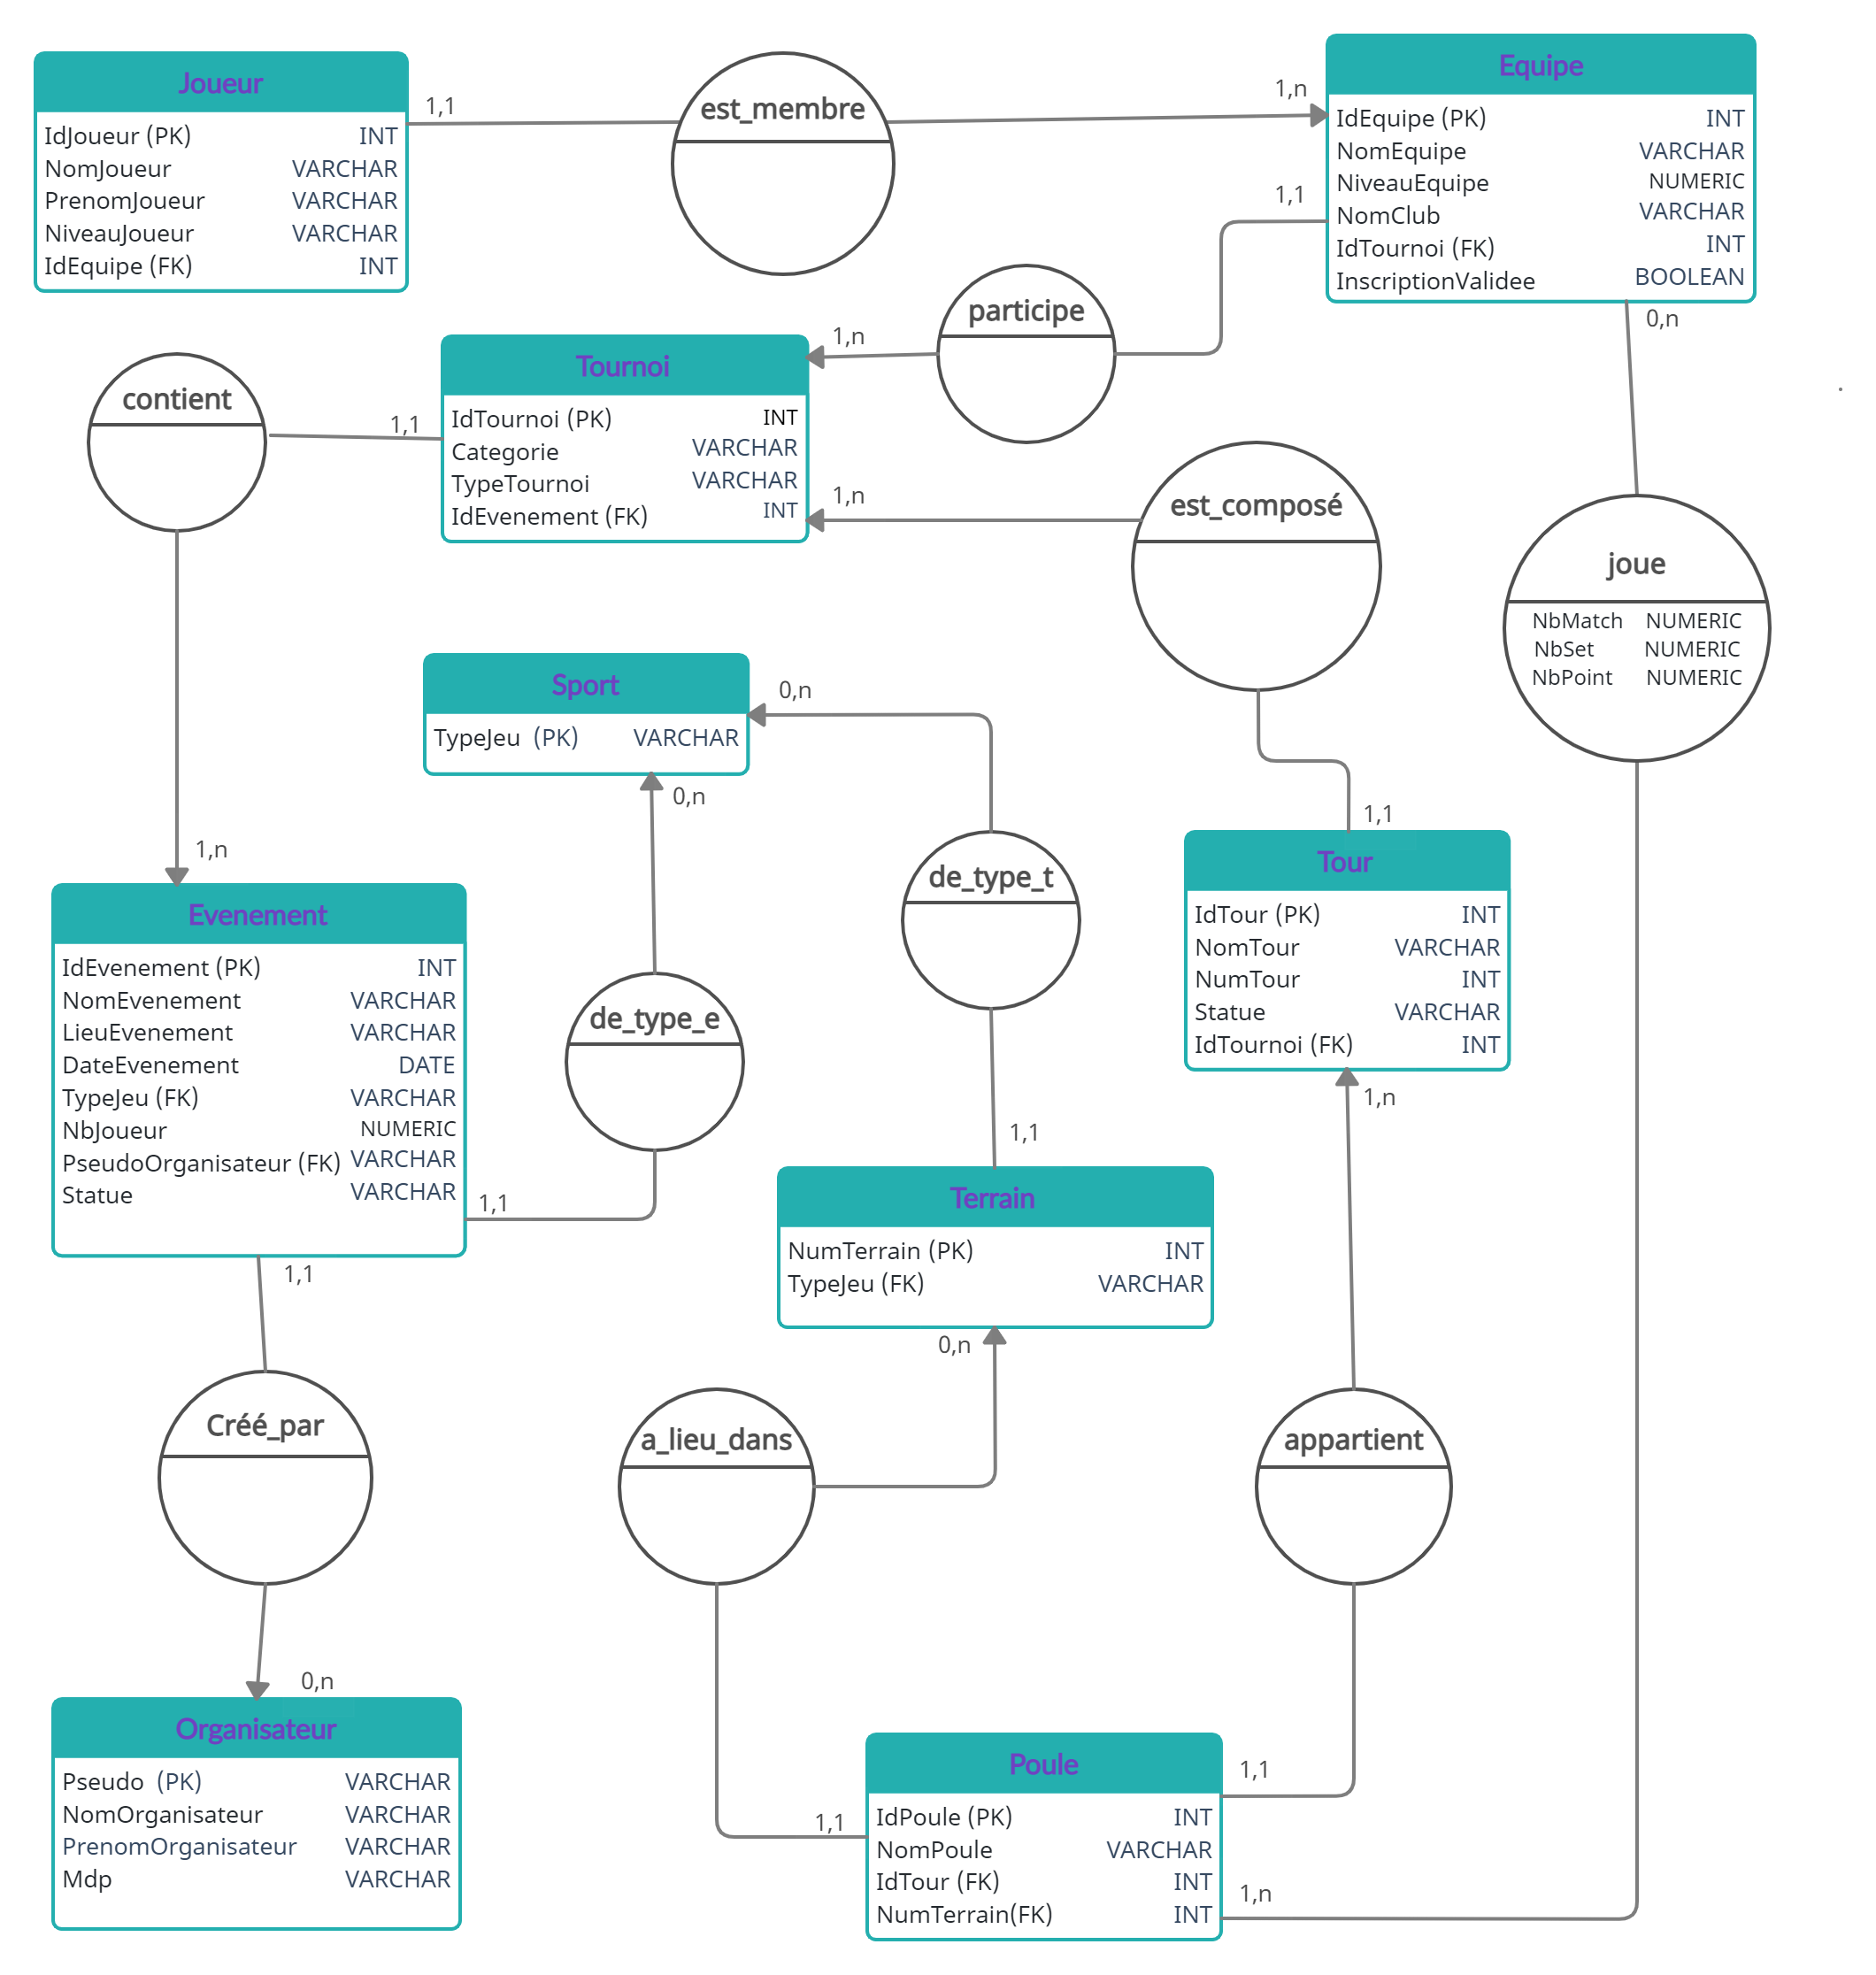
\includegraphics[height=17.5cm,width=17cm]{EA.png}
    \end{figure}
\end{center}
 
 
\section*{Explications}
\addcontentsline{toc}{section}{Explications}
\vspace{.5cm}
\subsection*{Entités}
\addcontentsline{toc}{subsection}{Entités}

\vspace{.5cm}


\begin{description}

\item[Organisateur:] C'est la personne qui a le droit de créer et d'éditer les événements. Il est identifié par son pseudo et possède un nom, un prénom et un mot de passe. \\

\item[Evenement:] Un événement est identifié par un id attribué. Il possède un nom, un lieu, une date, un type de jeu (sport), un nombre de joueur, le pseudo de son créateur et un statut. Le statut indique si l'événement n'a pas encore commencé, avait déjà commencé ou avait déjà terminé.\\

\item[Tournoi:] Un tournoi est identifié par un id attribué. Il possède une catégorie (initial, féminin, jeune...etc) et un type (principal ou consultante).\\

\item[Equipe:] Un équipe est identifié par un id attribué. Il possède un nom, un niveau, un nom de club et un attribut indiquant l'état de l'inscription de l'équipe. Cette entité représente une inscription d'équipe dans un tournoi. Le nom d'équipe est donc unique seulement dans ce tournoi. Deux équipes inscrits dans deux tournoi différents peuvent avoir le même nom.\\

\item[Joueur:] Un joueur est identifié par un id attribué. Il possède un nom, un prénom et un niveau.\\

\item[Tour:] Un tour est identifié par un id attribué. Il possède un nom, un numéro (pour conserver l'ordre) et un statut.\\

\item[Poule:] Une poule est identifiée par un id attribué et possède un nom.\\

\item[Terrain:] Un terrain est identifiée par un numéro attribué. Cette entité aurait pu être remplacée par un attribut directement intégré dans l'entité poule. Toutefois, avoir une entité terrain permet de spécifier le type de sport de chaque terrain ainsi que de chercher tous les terrains disponibles pour un sport choisi.\\

\item[Sport:] Un sport est identifiée par son nom. Cette entité aurait pu être remplacée par un attribut directement intégré dans l'entité événement. Toutefois, avoir une entité sport permet d'accéder directement aux sports qui sont reconnus et donc d'éviter d'avoir des problèmes comme (football, Football, FootBall...etc).
\\

\end{description}


\subsection*{Associations}
\addcontentsline{toc}{subsection}{Associations}


\vspace{.5cm}


\begin{description}

\item[Créé\_par:] Une association binaire entre Organisateur et Evenement. Un organisateur peut créer aucun ou plusieurs événements, et un événement est créé par un seul organisateur.\\

\item[Contient:] Une association binaire entre Evenement et Tournoi. Un Evenement contient au moins un tournoi, et un tournoi appartient à un seul événement. \\

\item[Participe:]Une association binaire entre Equipe et Tournoi. Un équipe peut participer dans exactement un tournoi, et un tournoi a au moins un équipe participant.\\

\item[Est\_membre:] Une association binaire entre Equipe et Joueur. Un équipe doit avoir au moins un joueur, et un joueur est membre d'un seul équipe.\\

\item[Est\_composé:] Une association binaire entre Tournoi et Tour. Un tournoi est composé d'au moins un tour, et un tour appartient à un seul tournoi.\\

\item[Appartient:] Une association binaire entre Tour et Poule. Un tour contient au moins une poule, et une poule appartient à un seul tour.\\

\item[Joue:] Une association binaire entre Equipe et Poule. Un équipe joue dans aucune ou plusieurs poules, et une poule contient au moins un équipe.\\

\item[A\_lieu\_dans:] Une association binaire entre Poule et Terrain. Une poule a lieu dans un terrain, et un terrain peut être utilisée par aucune ou plusieurs poule mais pas simultanément.\\

\item[de\_type\_t:] Une association binaire entre Terrain et Sport. Un terrain a un seul type de sport, et un sport peut avoir aucun ou plusieurs terrains.\\

\item[de\_type\_e:] Une association binaire entre Evenement et Sport. Un événement a un seul type de sport, et un sport peut avoir aucun ou plusieurs événements.\\

\end{description}

\chapter*{Modèle relationnelle}
\addcontentsline{toc}{chapter}{Modèle relationnelle}

\vspace{.5cm}

\begin{flushleft}
\begin{description}

\item[Organisateur](\underline{Pseudo}, NomOrganisateur, PrenomOrganisateur, Mdp).
\vspace{.3cm}
\item[Evenement](\underline{IdEvenement}, NomEvenement, LieuEvenement, DateEvenement, \textit{TypeJeu}, NbJoueur, \textit{PseudoOrganisateur},Statue).
\vspace{.3cm}
\item[Tournoi] (\underline{IdTournoi}, Categorie, TypeTournoi, \textit{IdEvenement}).
\vspace{.3cm}
\item[Equipe] (\underline{IdEquipe}, NomEquipe, NiveauEquipe, NomClub, \textit{IdTournoi}, InscriptionValidee).
\vspace{.3cm}
\item[Joueur] (\underline{IdJoueur}, NomJoueur, PrenomJoueur, NiveauJoueur, \textit{IdEquipe}).\\
\vspace{.3cm}
\item[Tour] (\underline{IdTour}, NomTour, NumTour, Statue, \textit{IdTournoi}).
\vspace{.3cm}
\item[Poule] (\underline{IdPoule}, NomPoule, \textit{IdTour}, \textit{NumTerrain}).
\vspace{.3cm}
\item[Joue] (\underline{\textit{IdPoule}, \textit{IdEquipe}}, NbMatch, NbSet, NbPoint).
\vspace{.3cm}
\item[Terrain] (\underline{NumTerrain}, \textit{TypeJeu}).
\vspace{.3cm}
\item[Sport] (\underline{TypeJeu}).


\end{description}
\end{flushleft}


\chapter*{Programmation procédurale}
\addcontentsline{toc}{chapter}{Programmation procédurale}

\section*{Triggers}
\addcontentsline{toc}{section}{Triggers}

\subsubsection*{Equipe\_Inscription\_Annulee}
\addcontentsline{toc}{subsection}{Equipe\_Inscription\_Annulee}
Ce trigger est déclenché après chaque modification d'un événement. Si l'événement a déjà commencé, il va supprimer tous les équipes qui n'ont pas encore validé leur inscription. 
\begin{center}
	\begin{figure}[!h]
          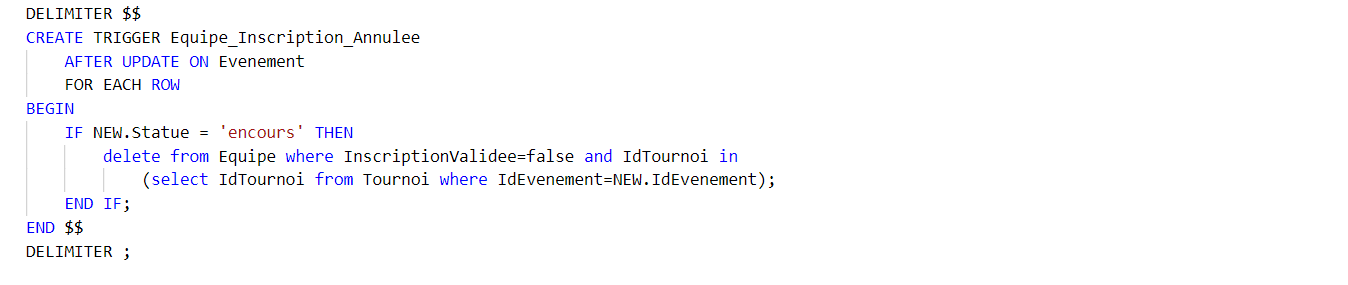
\includegraphics[width=24cm]{trigger1}  
    \end{figure}
\end{center}
 
\subsubsection*{Liberer\_Terrain}
\addcontentsline{toc}{subsection}{Liberer\_Terrain}
Ce trigger est déclenché après chaque modification d'un tour. Si le tour a déjà terminé, il va libérer tous les terrains qui étaient utilisés par les poules de ce tour. 
\begin{center}
	\begin{figure}[!h]
          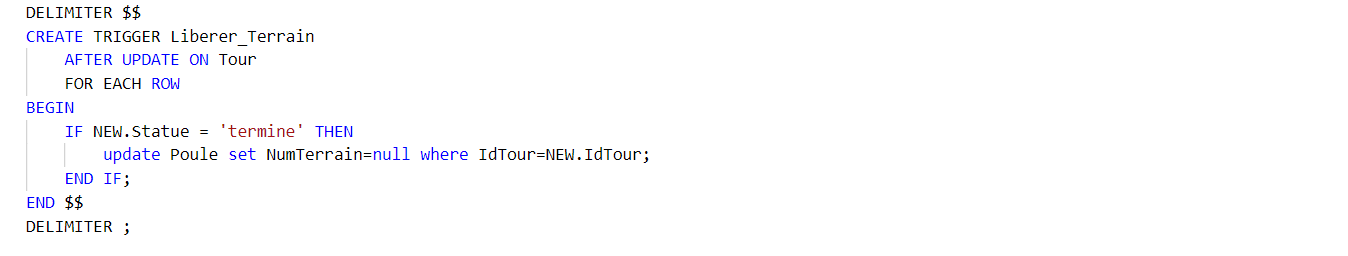
\includegraphics[width=24cm]{trigger2}  
    \end{figure}
\end{center}


\section*{Fonctions}
\addcontentsline{toc}{section}{Fonctions}
\subsubsection*{Get\_Classement}
\addcontentsline{toc}{subsection}{Get\_Classement}
Cette fonction prend en paramètre un id d'équipe et renvoie son classement dans le tournoi en tenant compte de tous les matchs, les sets et les points qu'il a gagné depuis le début du tournoi. Elle renvoie NULL si les matchs de ce tournoi n'ont pas encore commencé. 
\begin{center}
	\begin{figure}[!h]
          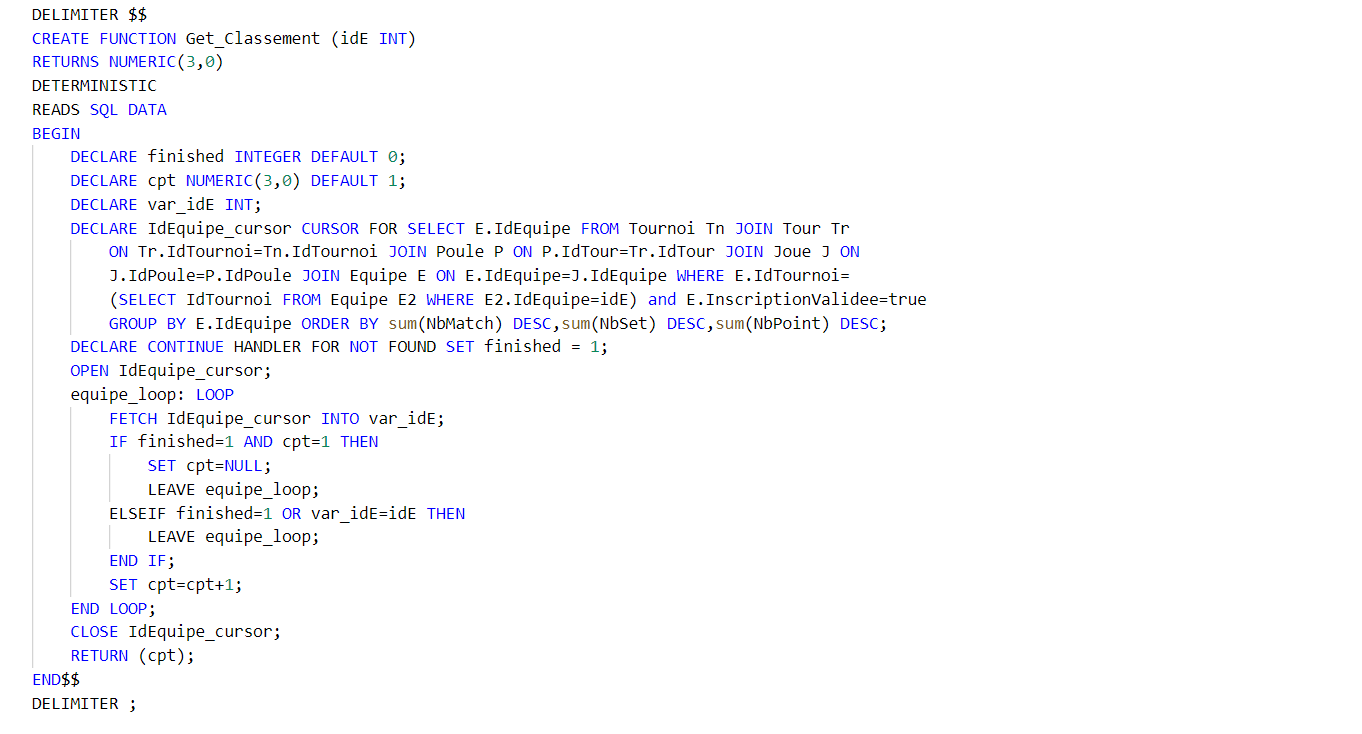
\includegraphics[width=24cm]{fonction}  
    \end{figure}
\end{center}

\newpage

\section*{Procédures}
\addcontentsline{toc}{section}{Procédures}
\subsubsection*{Remove\_Old\_Event}
\addcontentsline{toc}{subsection}{Remove\_Old\_Event}
Cette procédure supprime les événements qui n'ont toujours pas commencé alors que leur date a déjà dépassé la date d'aujourd'hui.
\begin{center}
	\begin{figure}[!h]
          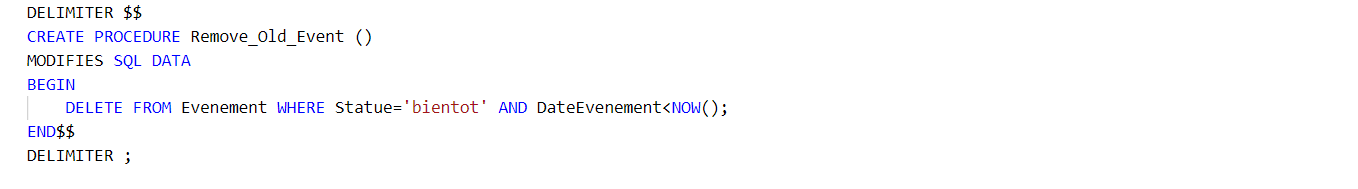
\includegraphics[width=24cm]{procedure}  
    \end{figure}
\end{center}



\section*{Événements}
\addcontentsline{toc}{section}{Événements}
\subsubsection*{Daily\_Remove\_Old\_Event}
\addcontentsline{toc}{subsection}{Daily\_Remove\_Old\_Event}
Cet événement est programmé pour appeler chaque jour la procédure \textit{Remove\_Old\_Event}. Cela garantit que tout événement ayant dépassé sa date sans commencer sera automatiquement supprimé de la base de données.
\begin{center}
	\begin{figure}[!h]
          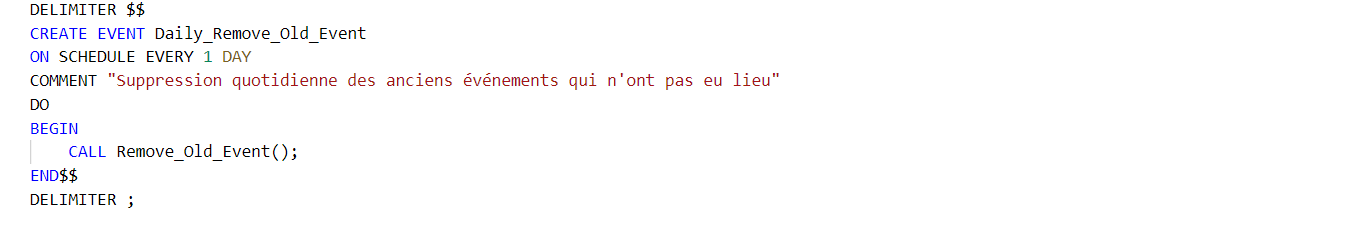
\includegraphics[width=24cm]{event}  
    \end{figure}
\end{center}



\end{document}